\documentclass[10pt,twocolumn,letterpaper]{article}

\usepackage{cvpr}
\usepackage{times}
\usepackage{epsfig}
\usepackage{graphicx}
\usepackage{amsmath}
\usepackage{amssymb}
\usepackage{float}
\usepackage{mathtools}
\usepackage{subcaption} 
\DeclarePairedDelimiter{\ceil}{\lceil}{\rceil}

% Include other packages here, before hyperref.

% If you comment hyperref and then uncomment it, you should delete
% egpaper.aux before re-running latex.  (Or just hit 'q' on the first latex
% run, let it finish, and you should be clear).
\usepackage[breaklinks=true,bookmarks=false]{hyperref}

\cvprfinalcopy % *** Uncomment this line for the final submission

\def\cvprPaperID{****} % *** Enter the CVPR Paper ID here
\def\httilde{\mbox{\tt\raisebox{-.5ex}{\symbol{126}}}}

% Pages are numbered in submission mode, and unnumbered in camera-ready
% \ifcvprfinal\pagestyle{empty}\fi
\begin{document}

%%%%%%%%% TITLE
\title{
    DeepCube: Transcribing Rubik's Cube Moves with Action Recognition
}

\author{Junshen Kevin Chen\\
Stanford University\\
{\tt\small jkc1@stanford.edu}
\and
Wanze Xie\\
Stanford University\\
{\tt\small wanzexie@stanford.edu}
\and
Zhouheng Sun\\
Stanford University\\
{\tt\small sunz@stanford.edu}
}

\maketitle

%%%%%%%%% ABSTRACT
% \begin{abstract}
%   The ABSTRACT is to be in fully-justified italicized text, at the top
%   of the left-hand column, below the author and affiliation
%   information. Use the word ``Abstract'' as the title, in 12-point
%   Times, boldface type, centered relative to the column, initially
%   capitalized. The abstract is to be in 10-point, single-spaced type.
%   Leave two blank lines after the Abstract, then begin the main text.
%   Look at previous CVPR abstracts to get a feel for style and length.
% \end{abstract}

%%%%%%%%% BODY TEXT
\section{Introduction}

% \textit{Introduction: this section introduces your problem and the overall plan for approaching your problem}

% \textit{Problem statement: Define your problem precisely, including inputs and outputs of your method.}

\paragraph{Motivation}
Speedcubing, namely solving a Rubik's Cube as fast as possible, has been a long standing sport since its invention. Currently, it often takes human effort to watch videos of cube solves, and transcribe the moves manually into text, and submit the solution sequence to speedcubing communities such as CubeSolves \cite{CubeSolves}, in order to conduct analysis of solves. With recent advance in video understanding and action recognition, we hypothesize that the process of manually transcribing Rubik's Cube moves can be automated using vision-based deep learning approaches. 

Furthermore, while action recognition has been popular and successful in detecting various human activities \cite{charades, ava, kinetics, finegym, hvu}, studies on the fine-grained atomic actions has been relatively scarce, mainly due to the lack of well-defined atomic activities. This motivates the problem of action recognition for Rubik's Cube operations, a subtle and atomic activity that is more challenging to detect.

With our work, we hope to facilitate speedcubing as a sport as well as push forward the frontier of vision-based fine-grained atomic action recognition.

\vspace{-2mm}
\paragraph{Problem formulation}
We formulate this problem as a \textbf{time-distributed multi-class classification} task. In this project, we aim to produce a model that takes input of a video clip of arbitrary length, and produce an output sequence of the same length, each element denoting one action completed at that time step, including "no action". 

% Although our vision is to enable reconstructing rubik's moves from any view angle under unconstrained backgrounds, it is limited by the difficulty to collect sufficient video data while preserving diversity of the background and viewing angles. 

To solve this problem, we introduce DeepCube, an egocentric video dataset of a person turning a Rubik's Cube under constrained environment. Our dataset is collected by 3 of us in well-lit environments with static monotonic background (see fig \ref{fig:recording_setup}). It contains 3 hours of recordings and have well distributed variety of cube moves including rotation and layer turns. To demonstrate the utility of the DeepCube dataset, we explore various methods \cite{lrcn,i3d,r3d} to tackle the task of action classification.

\section{Related Work}

While there exists a few research that explores the marriage between rubik's cube and deep learning \cite{cube_robotics, cube_rl}, they are related to constructing solution based on cube's current state with reinforcement learning \cite{cube_rl} and robotics \cite{cube_robotics}. Our work differs in that we want to detect cube's moves rather than constructing solution for it. Therefore our inspirations primarily draw from action recognition in videos. 
\vspace{-2mm}

\paragraph{Action recognition datasets.} Previously, most action recognition datasets focus on video classification, such as hollywood2 \cite{hollywood2}, UCF101 \cite{ucf101}, and YouTube-8M \cite{youtube8m}. These datasets are suited for tasks that directly maps the whole video clip to an action class. More recently, more works shift toward to temporal localization for activities. The datasets like Charades \cite{charades} and ActivityNet \cite{activitynet} contains long videos 
with multiple actions occurring at different time period. AVA \cite{ava} steps further and introduces spatio-temporal localization of actions and highlights the concept of atomic actions. Although most of the aforementioned datasets are allocentric, there exist a few egocentric video datasets like Something-something \cite {sthsth} and EPIC-Kitchens \cite{epic_kitchen}, but none focuses on atomic visual activities. This is where our work fits in - an egocentric video datasets for temporal atomic action localization in a specific task.

% We find Talk about atomic datasets like AVA, FineGym, also talk about egocentric dataset like something-something and epic kitchen.
\vspace{-2mm}

\paragraph{Action classification and localization.} Despite some non deep learning-based works \cite{sadek2012fast, stochastic}, a vast majority of action models with impressive results come from architecture that leverages CNN and RNN modules. One popular structure involves using CNN to extract visual features and feed into an RNN module for sequence learning, which allows variable-length visual input and class label output, known as LRCN \cite{lrcn}. Some modern state-of-the-art models \cite{ava, better_ava} often combines a "backbone" 3D CNN, such as I3D \cite{i3d} and R3D \cite{r3d}, with a region detector using Faster R-CNN \cite{faster_rcnn}, followed by a classifier to predict the action. One distinction in our task is that we put further emphasis on the order of the predicted action sequence, as one mistake in the order causes significant difference in the cube state of next moves.

% Talk about the usual state-of-the-art architecture like in LFB, introduced in AVA, better AVA. Also talk about Temporal Segment Networks, S3D. highlight that we do not need long-term feature for this work.

% \textit{The report should contain at least 3 references: they should not be generic CNN/deep learning references, but sources related to your project that you have read carefully. Describe briefly how each reference relates to your project.}

\section{Data}

% \textit{Clearly describe the dataset and any pre-processing steps. If you are collecting your own dataset or your project requires significant effort in data preprocessing, describe your work on the dataset collection / pre-processing pipeline clearly in a standalone subsection.}

We collect our own original dataset. We first present the format of our data, and then describe the collection process.

\paragraph{Format} 
The entire dataset is a collection of annotated video clips. For each video clip, we annotate each frame with a single label describing the move, from the following three categories:
\begin{enumerate}
    \item \textit{Zero label}, which means there is no action. 
    \item \textit{Layer-move labels}. These describe a 90-degree turn of one of the six outer layers of the cube, clockwise or counterclockwise. There are 12 possible labels in total.
    \item \textit{Rotation-move labels}. These describe a whole-cube rotation relative to a base orientation which we set during calibration. We assume rotations only happen around the x, y or z axis, and could be 90 $\deg$ clockwise or counterclockwise, or 180 $\deg$. There are 9 possible labels in total. 
\end{enumerate}

\paragraph{Collection}
We record moves using a camera facing the cube from the general direction of the solver, such that only the up and front faces are visible most of the time. The solver proceeds to do regular scrambles and solves at medium speed, so that motion blur is minimized. 

\begin{figure}[H]
    \centering
    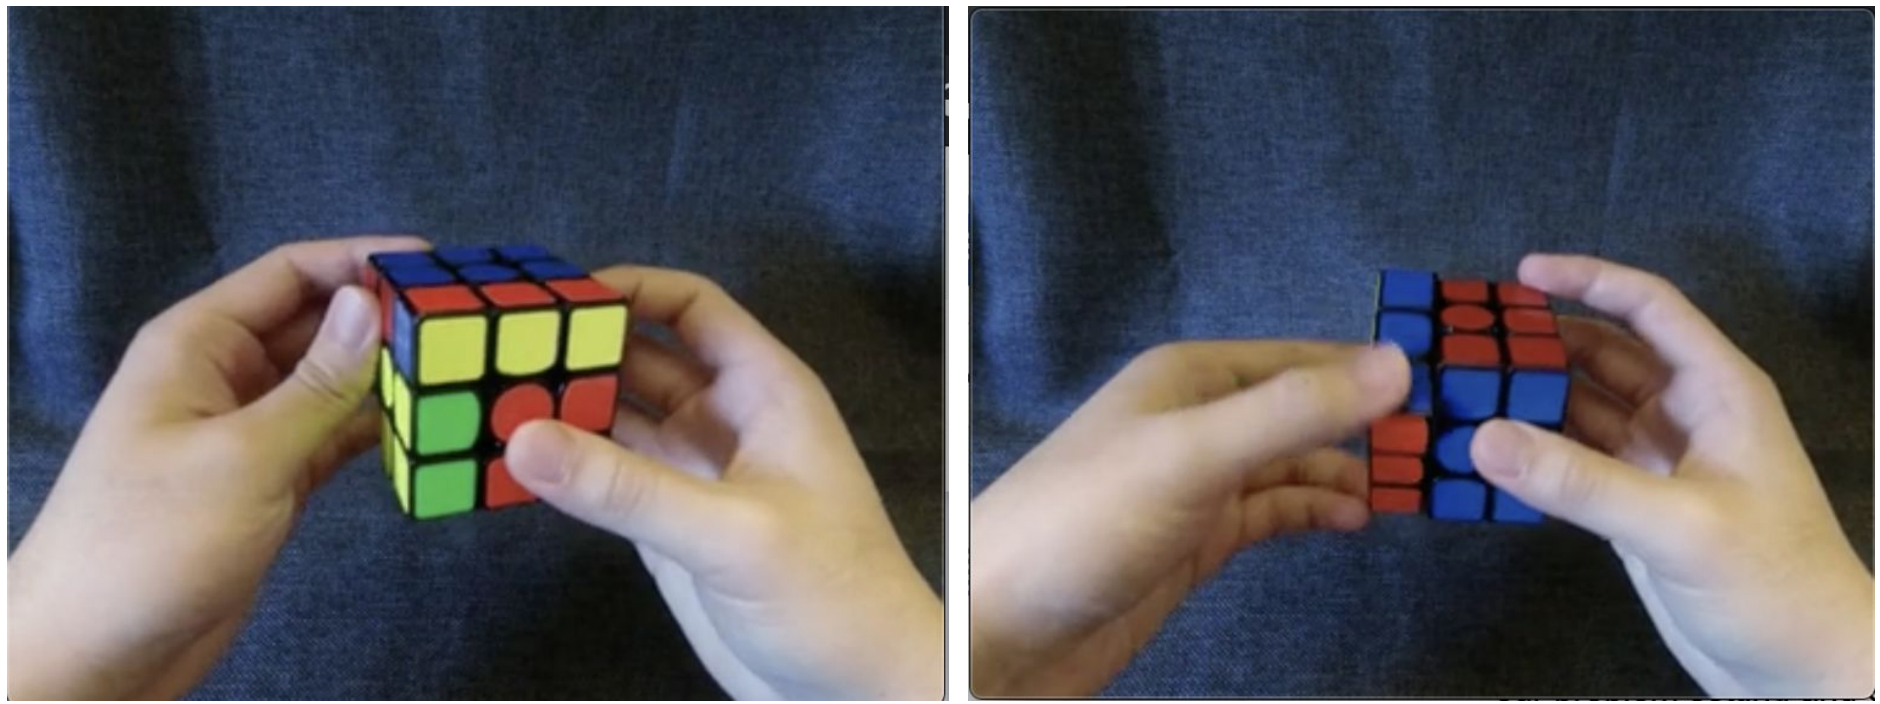
\includegraphics[scale=0.15]{recording_setup.png}
    \caption{Sample frames from our video dataset, and the right image is performing a move labeled as ‘L’.}
    \label{fig:recording_setup}
\end{figure}

To obtain the timestamp of each turn, we use commercial bluetooth-connected Rubik's Cube that emits signals for cube moves and orientations, sending a packet at \char`\~100ms intervals as soon as it detects an action is complete. We write a program that captures the signal while we are recording, and processes the signals to (timestamp, label) pairs. After recording finishes, we play the video and the annotation side by side, and manually align annotation timestamps with the video frames, so that the labels are aligned with the frame at which the move is considered finished by human viewers. 
 
In total there are more than 3 hours of video footage recorded at 30 fps, consisting of more than 20,000 layer and rotation moves in total.


\section{Methods}

% \textit{You should describe your method in concrete but concise technical detail, using equations or figures if necessary.
% In addition to the method you are proposing, the report should clearly describe one or more baseline methods you are comparing with, preferably in a separate subsection.
% Clearly specify the inputs and outputs of your method and the baseline method(s).}

\subsection{Input and Output}

\paragraph{Input} The input to the model are sequences of frames from the recorded video, which we down-sample to be 90 pixels wide and 68 pixels high, in 3 channels of RGB.

\paragraph{Output} The output of the model is a sequence of labels corresponding to each frame from the input, semantically denoting "which action \textbf{has finished} performing at this frame". Possible actions are:
\begin{itemize}
    \item No action $\emptyset$
    \item Cube rotation, denoted as \texttt{x,y,z}, their counterclockwise counterparts \texttt{x',y',z'}, and their 180 degree counterparts \texttt{x2,y2,z2}
    \item Layer turns to the cube, denoted as \texttt{L,R,U,D,F,B}, their counterclockwise counterparts, while their 180 degree counterparts are simply consecutive repeats of itself requiring no new classes
\end{itemize}
As such, we formulate the problem as a multi-class classification task, with 22 classes.

\subsection{Baseline}

For the baseline model we propose a statistical approach based on frame differences, drawing inspiration from the model \cite{sadek2012fast}, which was originally designed to recognize human body actions.
For each frame, we get the pixel-by-pixel frame differences from the previous frame, and calculate statistical features such as the center of motion. Features from all the frames are concatenated and passed into a fully connected network. This method does not handle segmentation of moves on its own, so for the purpose of evaluation, we supply readily segmented sequences of 5 frames with a single label denoting the only move (or blank) within these 5 frames. We were not able to get a satisfying result, and we attribute this to the fact that the model was aimed at coarse-grained whole-body actions, and that their object of interest is single-colored so its contour is easily identified. In our model, we aim at hand movement which is much more fine-grained, so a few statistical features may be insufficient for the task. Moreover, this approach does not distinguish between frame difference caused by the shift of the cube pieces, or the shift of the hands. Therefore, we do not report result for this baseline, as we will switch to the more feature-rich, CNN-based approaches as baseline instead.


\subsection{3D Convolutional Action Classifier}

Intuitively, because each turn of the cube is spans only several dozen frames, and the motion itself is entirely local to these frames, while being completely independent to any motion before of after it, the model only need to predict any motion given a range of frames. 


Figure \ref{fig:single_conv3d} depicts one convolution module consisting of a 3D convolutional layer, batch normalization, leaky ReLU activation, and max pooling. Before applying the convolution, we always zero-pad the input sequence in the time dimension, depending on the kernel size in the time dimension, such that the output sequence (extracted features) has exactly as many frames as input. 


\begin{figure}[]
  \begin{subfigure}[b]{0.23\textwidth}
    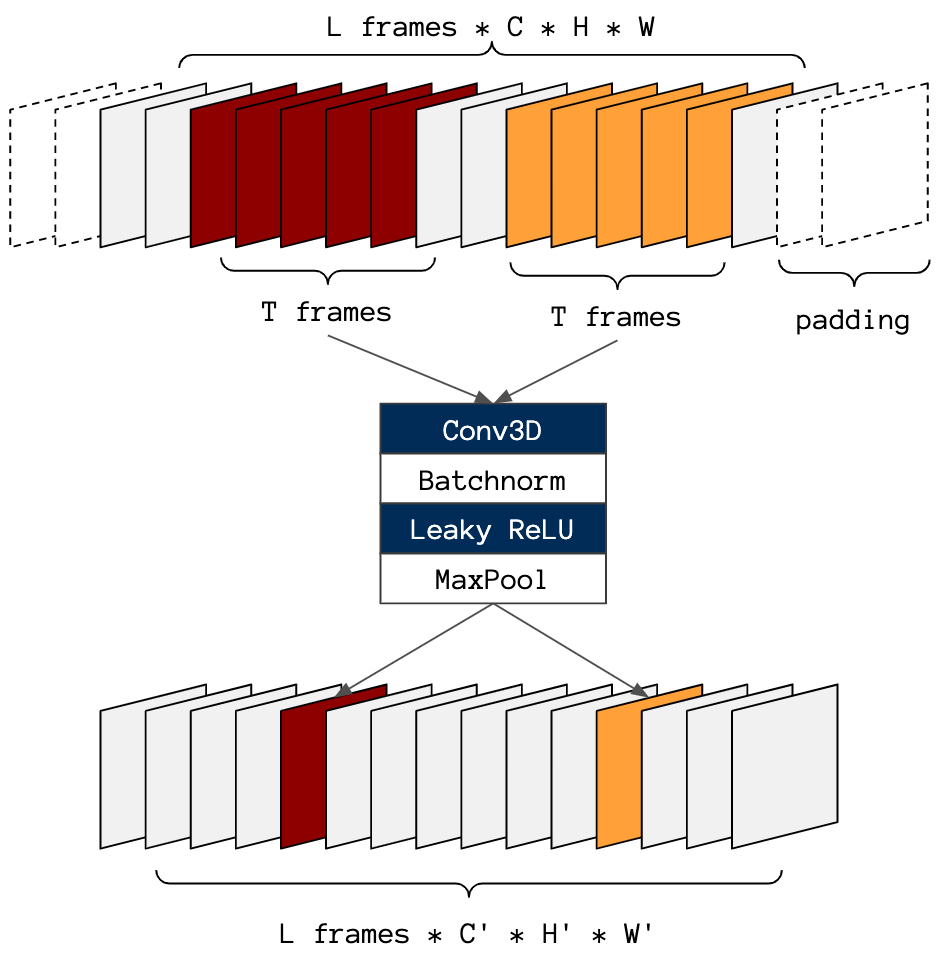
\includegraphics[width=\textwidth]{single_conv3d.png}
    \caption{Single 3D-conv module}
    \label{fig:single_conv3d}
  \end{subfigure}
  \begin{subfigure}[b]{0.23\textwidth}
    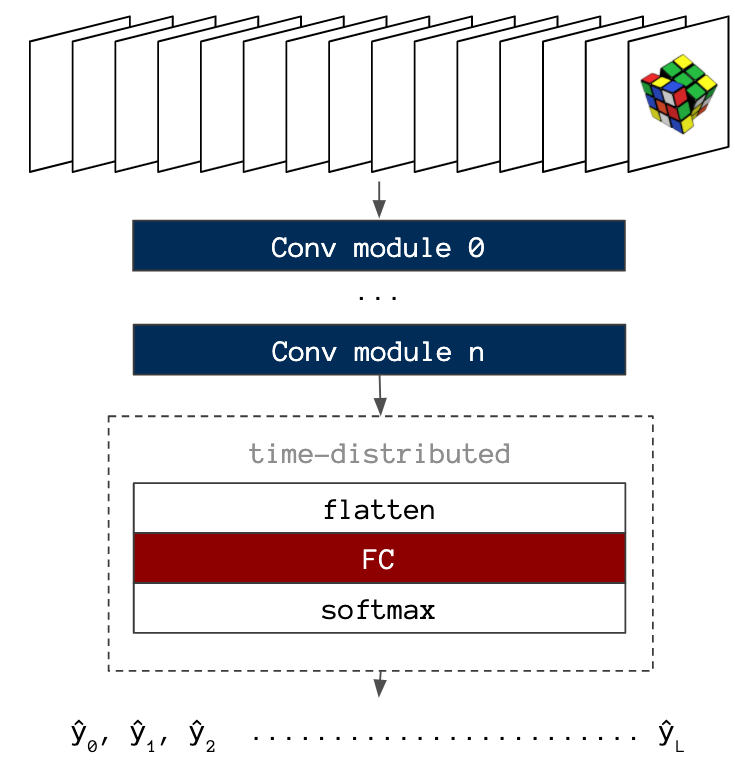
\includegraphics[width=\textwidth]{conv3d.png}
    \caption{3D-conv Classifier}
    \label{fig:conv3d}
  \end{subfigure}
  \caption{3D convolutional action classifier}
\end{figure}

After  one or more 3D convolutional modules (figure \ref{fig:conv3d}), we pass the extracted features into a module that flattens each frame, forward through a fully-connect network with ReLU activation, and finally a softmax activation to produce one predicted action per frame. This classification module is time-distributed, meaning that the same weights of the feed-forward network is applied equally to each frame over the time dimension. 

\subsection{3D-LRCN}

A 3D convolutional classifier has its field-of-view, including in the time dimension, defined as a hyperparameter of kernel size, stride, number of layers etc., so it is not suitable to learn the moves performed in different speed. For example, when the same move is conducted more quickly or slowly, the more than one convolution filter may need to be learned to capture the two types of fast and slow moves of the same kind. This is sub optimal, as outliers tend to cause incorrect predictions. 

To get around this problem, we may consider attaching the convolutional modules (ones before the time-distributed feed forward network) from the previous model, and use its extracted features to train a recurrent structure, namely an LSTM, to produce the predicted label, as depicted in fig \ref{fig:lstm}.

This is similar to LRCN \cite{lrcn}, which uses a 2D convolution feature extractor. Ideally, a 3D-LRCN should learn to observe each move, fast or slow, while building up an "activation energy", and when the move is complete, release the energy and produce a label, or predict 0 for all other time. 

\begin{figure}[]
    \centering
    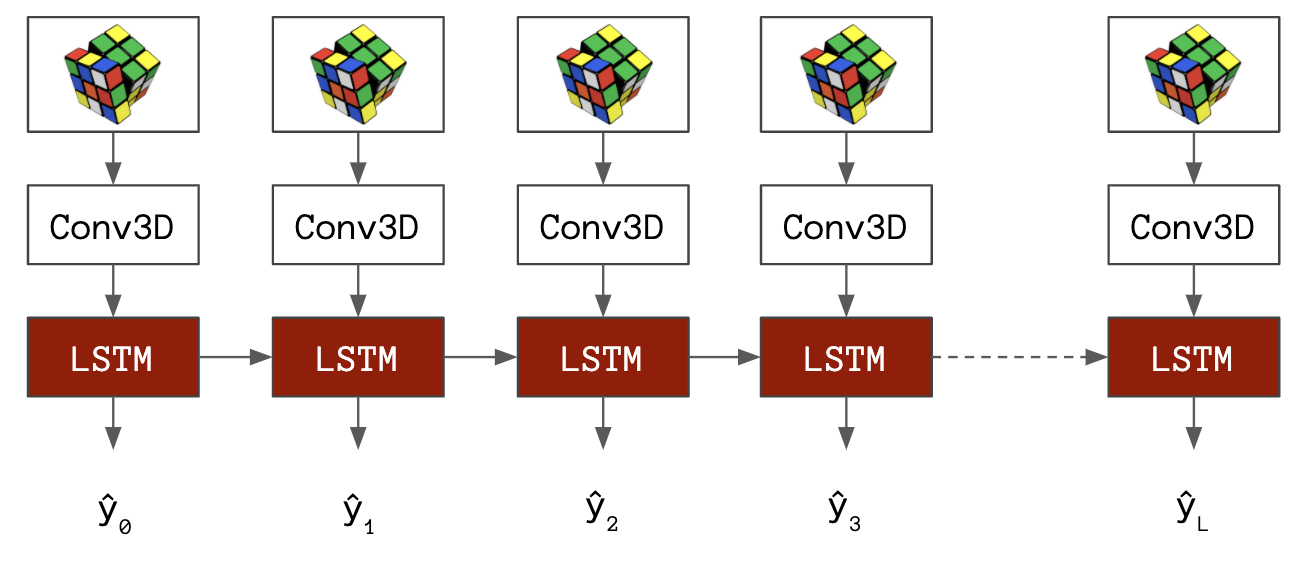
\includegraphics[scale=0.13]{lstm.png}
    \caption{LSTM module with 3D convolutional feature extractor.}
    \label{fig:lstm}
\end{figure}

\subsection{Collapsed Edit Distance}

The goal of this model is to transcribe the moves performed when given frames of videos, and therefore we should evaluate only on whether the predicted transcription is correct, i.e. the correct moves in the correct order. In our models, because we make a prediction in each timestep, and non-move is a valid prediction, we need to pre-process the output before evaluating the model.

The transcription of movement is \textbf{alignment-free}, meaning that it does not require an alignment between the input and the output strictly on each time step, it also does not require each move to only be predicted only one time step. We will collapse sequence by using the method identical to the one in Connectionist Temporal Classification (CTC) \cite{10.1016/j.neunet.2005.06.042}.

We perform this by merging repeats, and removing spaces, for both the prediction and the label \footnote{For ground truth label, we do not merge repeats, as they accurately denote repeated actions, we simple remove the spaces.}. Then, we take the edit distance, or how many insertion / modification / deletion it takes to edit one into another, between them as an evaluation metric of collapsed edit distance (CED).

For example:
\[
\hat{y} = [0,1,2,2,0,1], y = [0,0,0,1,0,0,0,2,1,1,0]
\atop 
Collapsed(\hat{y}) = Collapsed(y) = [1,2,1], 
CED(\hat{y}, y) = 0
\]


\section{Results}

% \textit{Quantitative evaluation results up to the milestone. The quantitative evaluation results should be in the form of figures or tables. All evaluation results should contain metrics other than loss values.}

At the time of drafting this report, our only working model is a 3D convolutional classifier, with 6 convolutional modules of conv3d-batchnorm-leakyrelu-maxpool3d, and a feed forward network of 512 hidden units. We evaluate on categorical cross entropy averaged for each time stamp, and collapsed edit distance averaged for each sequence of 100 frames. See table \ref{tab:best-model-stats}.




\begin{table}[]
\centering
\caption{3D convolutional classifier, mean metrics}
\label{tab:best-model-stats}
\begin{tabular}{rcc}
\hline
\multicolumn{1}{c}{}    & Train   & Dev     \\ \hline
Cross Entropy           & 0.20408 & 0.68143 \\
Collapsed Edit Distance & 1.28571 & 2.28643 \\ \hline
\end{tabular}
\end{table}

We observe some discrepancy between train and dev metrics, meaning that the model is not being descriptive enough to learn the pattern from training data, such that dev loss is significantly higher than train loss. This is also likely due to the abundance of saddle points in the optimization problem, as we observe the model takes more than 10 epochs before showing any significant loss decrease.

Qualitatively, we dive into the predicted label and noticed a pattern. When the labeled action is for example $[0,0,2,0,0]$, the model has the tendency to predict $[0,2,2,2,0]$, which is accurate after collapsing. However, this signals that the 3D-conv model is not being very effective in learning "what movement has \textbf{finished}", but rather "what movement \textbf{is happening}". This is likely due to the limitation of a convolutional structure, and the drawback of stacking many modules on top of each other that increases the perceptive field across the time dimension.

This leads to a problem of incorrect collapse when handling consecutive motions, for example when the labeled action is $[0,0,2,0,2,0]$ and the model predicts $[0,0,2,2,2,0]$, the collapsed result are not identical. We hope that using a recurrence on top of the convolutional structure can help solve this problem.

\section{Future Work}

\paragraph{More evaluation metrics.} So far, we mainly adopted edit distance as the quantitative metric for reasons we stated above. But in standard activity recognition tasks, mean average precision (mAP) is a more commonly used metric. Therefore, we look to evaluate our multi-class classification task using mAP. Similarly, since we also plan to implement temporal action localization using more modern architectures \cite{ss-tad, g-tad}, mAP will be the metric for this task as well.

\paragraph{3D-LRCN} The 3D-LRCN model is under active development, and we will experiment with different training methods to evaluate the results. 

\paragraph{3D-ResNet for action classification.} Although 3D CNN has showed some preliminary result for classification, our current approach is frame-based, where each frame maps to an action label. We hope to explore the performance of our dataset, if we were to predict just one action label given the trimmed video. This intuitively should work better given the success of trimmed video action classification on many datasets. 


\paragraph{SS-TAD/G-TAD for temporal localization.} Temporal action localization is a more complex task than classification. Although our current frame-based approach is able to temporally localize the end point of the action, it is difficult to evaluate if the model has identified the frames that involves the action since collapsed edit distance removes all temporal signals. Therefore, we think it might be worth to explore the task of identifying start and end frames of the predicted action label using some modern temporal localization models like SS-TAD \cite{ss-tad} and G-TAD \cite{g-tad}.

\clearpage

{\small
\bibliographystyle{ieee_fullname}
\bibliography{egbib}
}

\end{document}
